%!TEX root = pfc-memoria.tex
%!TEX encoding = UTF-8 Unicode

\chapter{Planificación}

\epigraph{``El progreso no se consigue por la suerte o por accidente sino trabajando en uno mismo diariamente.''}{\textsc{Epictetus} (55--135)}

En este capítulo organizaremos el desglose de tareas para hacer una planificación de las mismas en el calendario.

\section{Metodología de trabajo}

Utilizaremos un modelo de ciclo de vida iterativo en espiral \citep{Boehm1988}, pero dividiendo el proceso en dos paquetes de trabajo:
\begin{enumerate}[WP1]
\item La lectura y estudio de la bibliografía sobre NLP y ML; y su parte de documentación en la memoria.
\item Estudio de bibliotecas y frameworks disponibles; y análisis, diseño, implementación y pruebas del software; y su parte de documentación en la memoria.
\end{enumerate}

\begin{figure}[htbp]
\centering
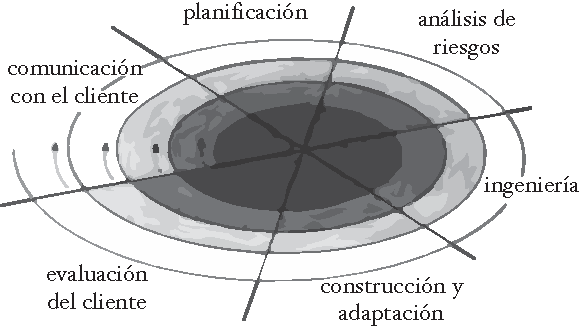
\includegraphics[width=0.55\textwidth]{espiral}
\caption[Modelo de ciclo de vida en espiral]{Modelo de ciclo de vida en espiral \citep{Boehm1988}}
\label{fig:espiral}
\end{figure}


\section{Planificación}

